\documentclass[12pt]{article}
\setlength\parindent{0pt}
\usepackage{amsmath}
\usepackage[margin=0.6in]{geometry}
\usepackage{graphicx}
\usepackage{fullpage}
\setlength{\parskip}{4mm}
\def\LL{\left\langle}   % left angle bracket
\def\RR{\right\rangle}  % right angle bracket
\def\LP{\left(}         % left parenthesis
\def\RP{\right)}        % right parenthesis
\def\LB{\left\{}        % left curly bracket
\def\RB{\right\}}       % right curly bracket
\def\PAR#1#2{ {{\partial #1}\over{\partial #2}} }
\def\PARTWO#1#2{ {{\partial^2 #1}\over{\partial #2}^2} }
\def\PARTWOMIX#1#2#3{ {{\partial^2 #1}\over{\partial #2 \partial #3}} }
\newcommand{\BE}{\begin{displaymath}}
\newcommand{\EE}{\end{displaymath}}
\newcommand{\BNE}{\begin{equation}}
\newcommand{\ENE}{\end{equation}}
\newcommand{\BEA}{\begin{eqnarray}}
\newcommand{\EEA}{\nonumber\end{eqnarray}}
\newcommand{\EL}{\nonumber\\}
\newcommand{\la}[1]{\label{#1}}
\newcommand{\ie}{{\em i.e.\ }}
\newcommand{\eg}{{\em e.\,g.\ }}
\newcommand{\cf}{cf.\ }
\newcommand{\etc}{etc.\ }
\newcommand{\Tr}{{\rm tr}}
\newcommand{\etal}{{\it et al.}}
\newcommand{\OL}[1]{\overline{#1}\ } % overline
\newcommand{\OLL}[1]{\overline{\overline{#1}}\ } % double overline
\newcommand{\OON}{\frac{1}{N}} % "one over N"
\newcommand{\OOX}[1]{\frac{1}{#1}} % "one over X"

\pagenumbering{gobble}

\begin{document}
\Large
\centerline{\sc{Lecture Tutorial -- Conservation of Energy}}

\normalsize

One of the most universal principles in physics is the {\it conservation of energy}. There are many kinds
of energy in nature; this tutorial will guide you through some reasoning
steps in applying the conservation of energy to what you've learned about planetary orbits.

This material {\it will} appear on the quiz; please ask questions if you have them.

Remember the overriding principle: {\it energy can't be created or destroyed}, only changed from one form
to another. This means that the total amount of energy in a system must stay constant.

The kinds of energy you need to worry about here are:

\begin{itemize}
\item {\bf Kinetic energy:} Energy associated with motion. Objects moving faster (or that are larger)
have more kinetic energy.

\item {\bf Gravitational potential energy:} Energy associated with an object's position near a large body that
attracts it. 

\item {\bf Other energy:} Heat, light, sound, and so on. These don't affect the orbits of the planets, but 
sometimes matter on Earth! Usually, friction winds up converting kinetic energy into sound and heat energy.

\end{itemize}

\Large 1. Falling on Earth
\normalsize

A bookshelf has two shelves. A red ball rests on the bottom shelf, which is one
meter off the ground; a green ball rests on the top shelf, which is two meters
off the ground. 
At some point, both fall off of their shelves and crash to the floor.

\begin{enumerate}

\item Do the balls have any kinetic energy when they are just sitting on the shelf?

\vspace{1in}

\newpage

\item 
As the balls fall, the
force of gravity accelerates them, and they move faster and faster. 
Energy can't be created or destroyed, only changed from one form to another. 

As they fall, the Earth's gravitational force accelerates them and makes them move faster and faster.
Since they are moving faster, they must be gaining kinetic energy. What kind of energy are they losing 
at the same time?

\vspace{1.5in}

\item Which ball has more kinetic energy right before it strikes the ground?
Explain your reasoning.

\vspace{1.5in}



\item Which ball started with more of the kind of energy you identified in part (2)? Explain your reasoning.
\newpage
\item Draw graphs of the amount of different kinds of energy that the balls have as they fall. You should
draw two lines on each set of axes, one for the red ball (falling off the short shelf) and one for the green ball (falling off the tall shelf).
\begin{center}

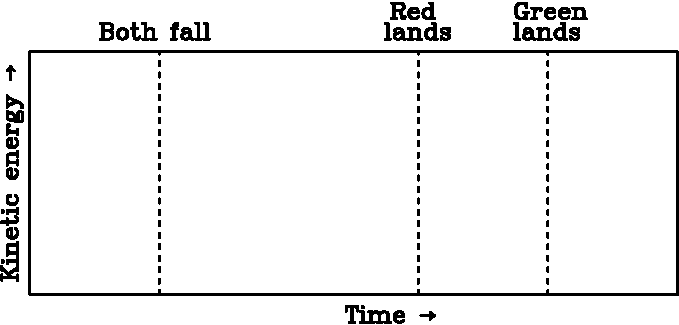
\includegraphics[width=0.6\textwidth]{kinetic-graph-1-crop.pdf}

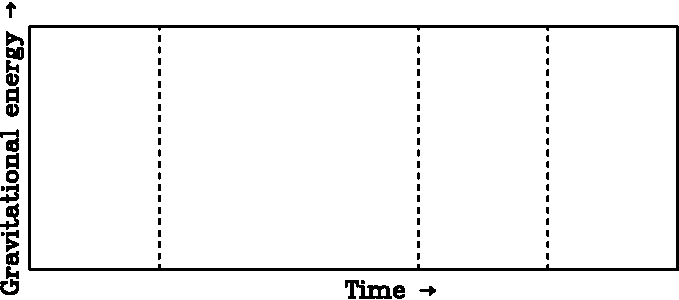
\includegraphics[width=0.6\textwidth]{gpe-graph-1-crop.pdf}

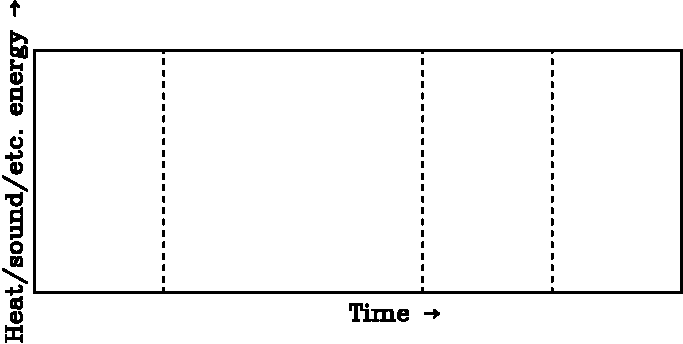
\includegraphics[width=0.6\textwidth]{other-graph-1-crop.pdf}

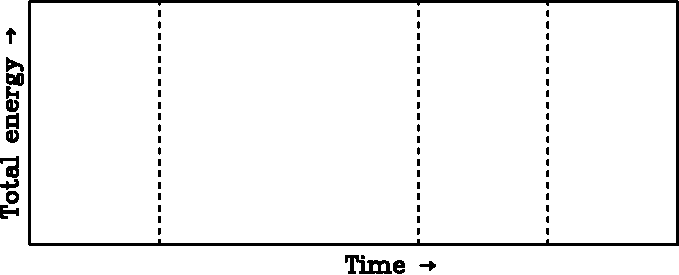
\includegraphics[width=0.6\textwidth]{total-graph-1-crop.pdf}

\end{center}

\newpage

\item Two students are debating the answers to the preceding.

\begin{itemize}
\item {\bf Student A:} After they have already hit the ground, they don't have any kinetic energy any more.
We also know gravitational potential energy is based on how high you are, and so they don't have any potential
energy either once they are lying on the floor. That means their total energy has to be zero. There might
be some sound energy as they go ``thump'', but that will only last for an instant.

\item {\bf Student B:} You're forgetting that there are other kinds of energy besides these.
It will probably heat the balls and the carpet up
by just a little bit. Just because we can't see it doesn't mean it's not there!

\end{itemize}

Who do you agree with, and why?

\end{enumerate}

\vspace{1in}

\Large 2. Falling in Astronomy \normalsize

In the previous question, you looked at conservation of energy as an object falls on Earth. The same ideas
apply in space; if anything, the situation in space is simpler.

Suppose you have an asteroid orbiting the Sun in an elliptical orbit as shown.

\begin{center}
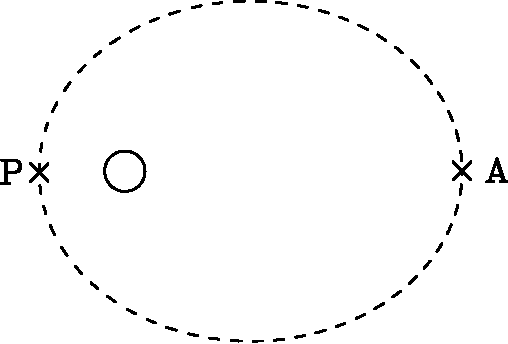
\includegraphics[width=0.5\textwidth]{orbit-crop.pdf}
\end{center}

The aphelion and perihelion (points furthest from and closest to the Sun) are labeled ``A'' and ``P''.

\begin{enumerate}

\item Is it correct to say that the asteroid, as it travels from aphelion to
perihelion, ``falls toward the Sun'' in some sense? Explain.

\vspace{1in}

\item In the last section, you saw that the green ball, on a tall shelf, had more gravitational potential
energy than the red ball, on a shelf closer to the ground.

Applying this idea to the orbit shown here, how does the {\it gravitational potential energy} of the asteroid
at perihelion compare to the gravitational potential energy at aphelion?

\vspace{1in}

\item How does the {\it total energy} of the asteroid
at perihelion compare to the gravitational potential energy at aphelion? (What do you know about the {\it total energy} of a system?)

\vspace{1in}

\item When the asteroid is moving closer to the Sun, its potential energy is \underline{\hspace{1in}}.
This means that its kinetic energy, and thus its speed, are \underline{\hspace{1in}}.

\item When the asteroid is moving {\it further} from the Sun, its potential energy is \underline{\hspace{1in}}.
This means that its kinetic energy, and thus its speed, are \underline{\hspace{1in}}.

\vspace{0.5in}

\item Kepler's second law says that the line connecting the asteroid to the Sun sweeps out equal areas in equal 
times. Is this a consequence of the conservation of energy? Explain your reasoning.

\newpage

Consider the exchange of energy between kinetic and potential as the asteroid orbits
the Sun twice, starting at aphelion. On the axes provided, draw graphs of the
different kinds of energy that the asteroid has at different points in its orbit.
Notice that the aphelion and perihelion points have been labeled.
\begin{center}

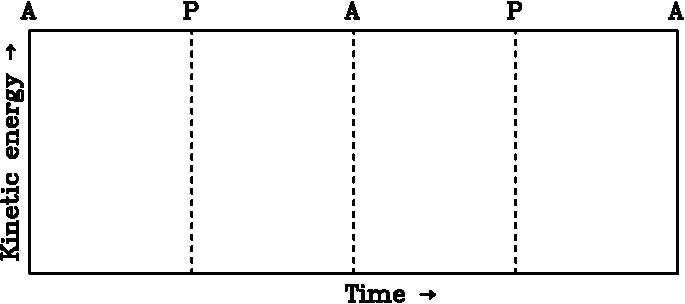
\includegraphics[width=0.6\textwidth]{kinetic-orbit-crop.pdf}

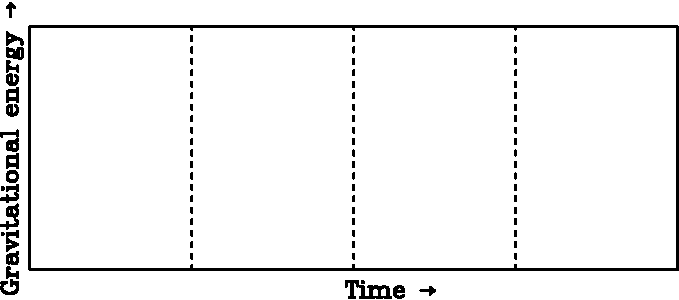
\includegraphics[width=0.6\textwidth]{gpe-orbit-crop.pdf}

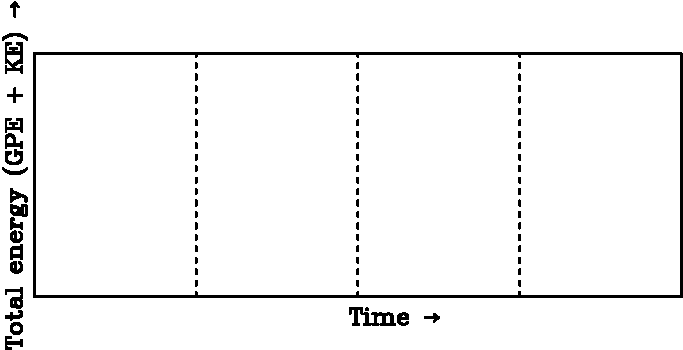
\includegraphics[width=0.6\textwidth]{total-orbit-crop.pdf}

\medskip

Here's the orbit again for reference:

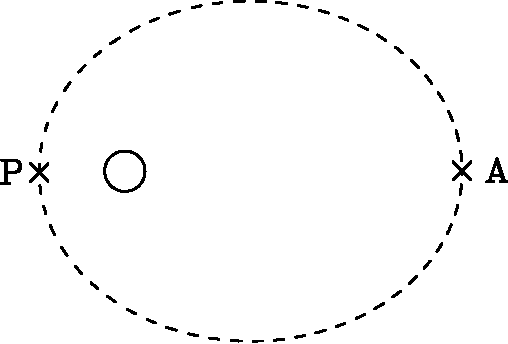
\includegraphics[width=0.35\textwidth]{orbit-crop.pdf}
\end{center}

\newpage
\item Our two favorite students, Student A and Student B, 
are debating their answers to the previous 
problem. Student C chimes in with a comment of their own.

\begin{itemize}

\item {\bf Student A:} I think the energy has to increase and decrease as the 
asteroid orbits. It's moving faster at perihelion, by Kepler's second law, and 
thus it has to have more energy there.

\item {\bf Student B:} Actually, it's the other way around. Think back to the balls on the
shelves. If the asteroid is at aphelion -- further from the Sun -- that's like 
being on the top shelf of the bookshelf, and we decided that it had more energy
{\it there}.

\item {\bf Student C:} Wait... isn't the total energy always the same? We know that
energy is never gained or lost, only converted from one form to another.

\end{itemize}

Who do you agree with, and why? Are multiple people correct?

\end{enumerate}
\end{document}
